\documentclass[11pt,letterpaper,boxed]{hmcpset}
\usepackage{fullpage}
\setlength{\parskip}{6pt}
\setlength{\parindent}{0pt}
\usepackage[margin=1in]{geometry}
\usepackage{graphicx}
\usepackage{enumerate}
\usepackage{marvosym}
\usepackage{amssymb}
\usepackage{wasysym}
\usepackage{gensymb}
\usepackage{mathrsfs}
\usepackage{scrextend}
\usepackage{mathtools}
\usepackage{pgfplots}
\usepackage{xspace}

\name{Name $\rule{4cm}{0.15mm}$}
\class{Physics 51M Section $\rule{.5cm}{0.15mm}$ Box \# $\rule{1cm}{0.15mm}$}
\assignment{Problem Set 1}
\duedate{9 September 2019}

\begin{document}
	
	%\begin{center}
	\noindent\textbf{Collaborators:} 
	%\end{center} 
	
	%\problemlist{}
	
	\begin{problem}[Schey I-1 (c,f,g)]
		Using arrows of proper magnitude and direction, sketch each of the following vector functions. \textbf{Check each answer using VectorFieldDemo.py program.}
		\begin{enumerate}
			\item[(c)] $\textbf{i}x - \textbf{j}y$
			\item[(f)] $(\textbf{i}y + \textbf{j}x)/\sqrt{x^2+y^2}$, $(x,y) \neq (0,0)$
			\item[(g)] $\textbf{i}y + \textbf{j}xy$
		\end{enumerate}
	
		\textbf{Professor note:} Please use $\hat x$, $\hat y$, and $\hat z$ unit vectors instead of $\hat i$, $\hat j$, and $\hat k$. The textbook uses math unit vectors, but we would like you to get out of this habit as soon as possible. 
		
	\end{problem}
	
	\begin{solution}
		\vfill
	\end{solution}
	\newpage
	
	
	\begin{problem}[Schey I-3]
		Check each answer using VectorFieldDemo.py program.
		\begin{enumerate}
			\item[(a)] Write a formula for a vector function in two dimensions which is in the positive radial direction and whose magnitude is 1.
			\item[(b)] Write a formula for a vector function in two dimensions whose direction makes an angle of $45^{\circ}$ with the $x$-axis and whose magnitude at any point $(x,y)$ is $(x+y)^2$.
			\item[(c)] Write a formula for a vector function in two dimensions whose direction is tangential (in the sense of the example on page 5) whose magnitude at any point $(x,y)$ is equal to distance from the origin.
			\item[(d)] Write a formula for a vector function in three dimensions which is in the positive radial direction and whose magnitude is 1.
		\end{enumerate}
		
		\textbf{Professor note:} Please use $\hat x$, $\hat y$, and $\hat z$ unit vectors instead of $\hat i$, $\hat j$, and $\hat k$. The textbook uses math unit vectors, but we would like you to get out of this habit as soon as possible. 
		
	\end{problem}
	
	\begin{solution}
		\vfill
	\end{solution}
	\newpage
	
	
	\begin{problem}[Schey I-5]
		A charge $+1$ is situated at the point $(1,0,0)$ and a charge $-1$ is situated at the point $(-1,0,0)$. Find the electric field of these two charges at an arbitrary point $(0,y,0)$ on the $y$-axis.
		\linebreak
		\newline
		\textbf{Professor note:} This is a mathematical formulation of a physics problem, so it is missing all the units. Please assume that the charges are in Coulombs and the lengths are in meters. 
			
	\end{problem}
	
	\begin{solution}
		\vfill
	\end{solution}
	\newpage
	
	
	\begin{problem}[HRK E25.7*]
		Three charged particles lie on a straight line and are separated by a distance $d$ as shown in Fig. 25-19. Charges $q_1$ and $q_2$ are held fixed. Charge $q_3$, which is free to move, is found to be in equilibrium under the action of the electric forces. Find $q_1$ in terms of $q_2$.
		
		\begin{center}
			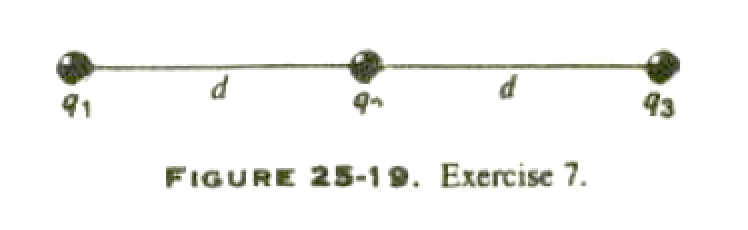
\includegraphics[scale=0.5]{25-19.png}
		\end{center}
		
	\end{problem}
	
	\begin{solution}
		\vfill
	\end{solution}
	\newpage
	
	\begin{problem}[HRK P25.10]
		In the compound CsCl (cesium chloride), the Cs atoms are situated at the corners of a cube with a Cl atom at the cube's center. The edge length of the cube is 0.40nm; see Fig. 25-23. The Cs atom carries one excess electron. 
		
		\begin{enumerate}
			\item[(a)] What is the strength of the net electric force on the Cl atom resulting from the eight Cs atoms shown? 
			\item[(b)] Suppose that the Cs atom marked with an arrow is missing (crystal defect). What now is the net electric force on the Cl atom resulting from the seven remaining Cs atoms?
		\end{enumerate}
	
		\begin{center}
			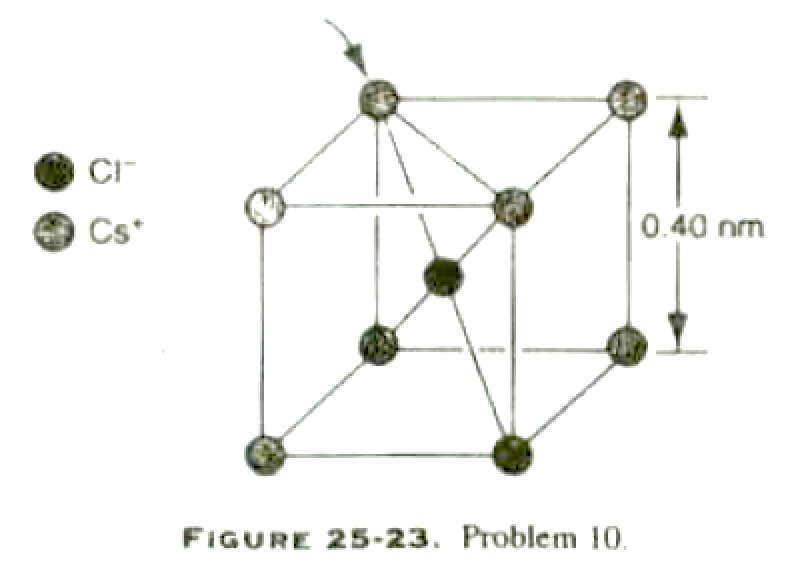
\includegraphics[scale=0.5]{25-23.png}
		\end{center}

	\end{problem}
	
	\begin{solution}
		\vfill
	\end{solution}
	\newpage
	
	\begin{problem}[HRK P25.11]
		Two equal positive point charges $q$ are held a fixed distance away $2a$ apart. A point test charge is located in a plane that is normal to the line joining these charges and midway between them. Find the radius $R$ of the circle in this plane for which the force on the test particle has a maximum value. See Fig. 25-24.
		
		\begin{center}
			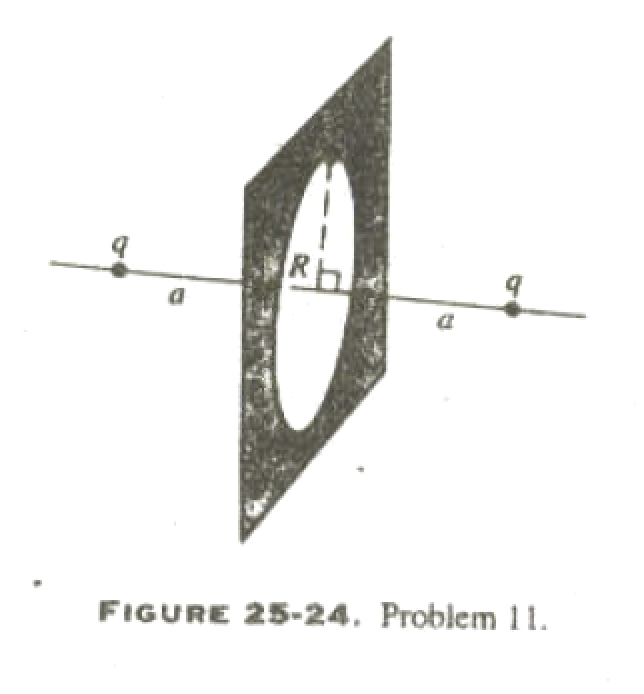
\includegraphics[scale=0.5]{25-24.png}
		\end{center}
		
	\end{problem}
	
	\begin{solution}
		\vfill
	\end{solution}
	
\end{document}